\documentclass[../main.tex]{subfiles}
\begin{document}
\section*{Problem Set 7}
    Name: Fangyuan Lin, UC Berkeley, Class of 2024
\subsection*{7.3 Memory increases capacity} Consider a binary symmetric channel with crossover probability $0<\epsilon < 1$ represented by $X_i=Y_i+Z_i\mod 2$, where $X_i,Y_i$ and $Z_i$ are respectively the input, output, and the noise variable at time $i$. Then \[
\Pr\{Z_i=0\}=1-\epsilon\quad \text{and}\quad \Pr\{Z_i=1\}=\epsilon
\] We assume that the input and the noise are independent, but we don't make the assumption that $Z_i$ are iid, meaning the channel may have memory.
\newline
a) Prove that \[
\I(\vec X;\vec Y)\leq n-h_b(\epsilon).
\]
\begin{proof}
    \begin{align*}
        I(\vec X,\vec Y)&=H(\vec Y)-H(\vec Y|\vec X)\\
        &\leq \sum_i H(Y_i)-H(\vec Y|\vec X) \quad \text{by independence bound}\\
        &= n-H(\vec Y|\vec X)\\
        &\leq n-h_b(\epsilon)
    \end{align*}
because  \begin{align*}
    H(\vec Y|\vec X)&=H(\vec X+\vec Z|\vec X)\\
    &=H(\vec Z|\vec X)\\
    &=H(\vec Z)\\
    &\geq H(Z_1)\\
    &=h_b(\epsilon)
\end{align*}
\end{proof}
b) Show that the upper bound in (a) can be achieved by letting $X_i$ be iid bits taking the values $0$ and $1$ with equal probability and $Z_1=Z_2=\dots=Z_n$.
\begin{proof}
    Since $Z=Z_1=\dots=Z_n$, we have that $H(\vec Z)=H(Z_1)$.
    \newline
    % Note that independence bound above is tight if and only if each $Y_i$ are iid. 
    Then we note that $Y_i$ are mutually independent because the $X_i$ are mutually independent.
    \end{proof}
c) Show that with the assumption in (b), $I(\vec X,\vec Y)>nC$, where $C=1-h_b(\epsilon)$ is the capacity of the BSC if it is memoryless.
\begin{proof}
    \begin{align*}
        I(\vec X,\vec Y)&=n-h_b(\epsilon)\\
        &>n(1-h_b(\epsilon))\\
        &=nC
    \end{align*}
\end{proof}

\subsection*{7.7 BSC with transition matrix}
Let \[
P(\epsilon)=\begin{bmatrix}
    1-\epsilon & \epsilon \\
    \epsilon & 1-\epsilon
\end{bmatrix}
\] be the transition matrix for a BSC with crossover probability $\epsilon$. Define $a*b=(1-a)b+a(1-b)$ for $0\leq a,b\leq 1$.
\newline
a) Prove that a DMC with transition matrix $P(\epsilon_1)P(\epsilon_2)$ is equivalent to a BSC with crossover probability $\epsilon_1*\epsilon_2$. Such a channel is the cascade of two BSCs with crossover probabilities $\epsilon_1$ and $\epsilon_2$, respectively.
\begin{proof}
    \begin{align*}
        &P(\epsilon_1)P(\epsilon_2) \\
        &=\begin{bmatrix}
            1-\epsilon_1 & \epsilon_1\\
            \epsilon_1 & 1-\epsilon_1
        \end{bmatrix}\begin{bmatrix}
            1-\epsilon_2 & \epsilon_2\\
            \epsilon_2 & 1-\epsilon_2
        \end{bmatrix}\\
        &=\begin{bmatrix}
            1-\epsilon_1 *\epsilon_2& \epsilon_1*\epsilon_2\\
            \epsilon_1*\epsilon_2 & 1-\epsilon_1*\epsilon_2\\
            &=P(\epsilon_1*\epsilon_2)
        \end{bmatrix}
    \end{align*}
    Just algebra.
\end{proof}
b) Repeat a) for a DMC with transition matrix $P(\epsilon_2)P(\epsilon_1)$. \begin{proof}
    Note that the $*$ operation defined above is commutative so \[
    P(\epsilon_2)P(\epsilon_1)=P(\epsilon_1)P(\epsilon_2),
    \]
    meaning that the order of the 2 channels does not matter.
\end{proof}
c) Prove that \[1-h_b(\epsilon_1 * \epsilon_2)\leq \min(1-h_n(\epsilon_1), 1-h_n(\epsilon_2)).
\] This means that the capacity of the cascade of 2 BSC's is upper bounded by the capacity of either of the 2 BSC's.
\begin{proof}
    This is an algebra problem. First, note that \[
    \epsilon_1 * \epsilon_2 = \epsilon_1 + \epsilon_2 -2\epsilon_1\epsilon_2
    \]
    We show that $\epsilon_1 * \epsilon_2$ is further away from $0.5$ then $\epsilon_1$ or $\epsilon_2$: \begin{align*}
        &(0.5-\epsilon_1 * \epsilon_2)^2-(0/5-\epsilon_1)^2\\
        &=-\epsilon_2(1-\epsilon_2 )(1-2\epsilon_1)^2\\
        &\leq 0
    \end{align*}
\end{proof}
d) Prove that a DMC with transition matrix $P(\epsilon)^n$ is equivalent to a BSC with crossover probabilities $\frac{1}{2}(1-(1-2\epsilon)^n)$
\begin{proof}
    Proof by induction. Assume the statement is true for $n=m$, then \begin{align*}
        &\epsilon^{(*m)}*\epsilon\\
        &=\frac{1}{2}(1-(1-2\epsilon)^{m+1}) \quad \text{algebra}
    \end{align*}
\end{proof}
\subsection*{7.8 Symmetric Channel} A DMC is symmetric if the rows of the transition matrix $p(y|x)$ are permutations of each other and so are the columns. Determine the capacity of such a channel.
\begin{proof}
    \begin{itemize}
        \item Note that $H(Y|X)=H(Y|X=x)$ for any $x$ because each row is the same distribution.
        \item If $X$ follows a uniform distribution on $\X$, then for each $y$, \[
        p(y)=\sum_xp(x)p(y|x)=\frac{1}{|\X|}\sum_xp(y|x)
        \], which does not depend on $y$ because columns are permutations of each other. 
    \end{itemize}
    \begin{align*}
       I(X;Y)&=H(Y)-H(Y|X)\\
       &=H(Y)-\sum_xp(x)H(Y|X=x)\\
       &=H(Y)-H(Y|X=x)\\
       &\leq \log|\Y|-H(Y|X=x)
    \end{align*}
    To achieve the upper bound, we let $Y$ follows a uniform distribution.
\end{proof}

\subsection*{7.9 Two channels in series - Bottleneck}
Let $C_1$ and $C_2$ be the capacities of 2 discrete memoryless channels with transition matrices $P_1$ and $P_2$ respectively. Let $C$ be the capacity of a DMC with transition matrix $P_1P_2$. Prove that \[
C\leq min(C_1, C_2).
\]
\begin{proof}
    We think of the new DMC as the 2 DMC's connected in series. Let $X$ denote the input random variable and let $Y$ denote the output obtained by passing the input though the DMC with transition matrix $P-1$. Let $Z$ denote the random variable obtained as the end. Then $X\to Y\to Z$ forms a Markov chain. Then by data processing inequality,
    \[
    C = \sup I(X;Z) \leq \sup I(X;Y) = C_1
    \] and 
    \[
    C = \sup I(X;Z) \leq \sup I(Y;Z) = C_2.
    \]
\end{proof}

\subsection*{7.10 Two channels in parallel} Let $C_1$ and $C_2$ be the capacities of two DMCs $p_1(y_1|x_1)$ and $p_2(y_2|x_2)$ respectively. Determine the capacity of the DMC \[
p(y_1,y_2|x_1,x_2) := p_1(y_1|x_1)p_2(y_2|x_2)
\] 
Hint: Prove that \[
I(X_1,X_2;Y_1,Y_2)\leq I(X_1,Y_1) + I(X_2,Y_2)
\] if $p(y_1,y_2|x_1,x_2) := p_1(y_1|x_1)p_2(y_2|x_2)$.
\begin{proof}
    Since $Y_1\to X_1\to X_2\to Y_2$ forms a Markov chain, we can see from information diagram that \[
    I(X_1;Y_1) + I(X_2;_2) = I(X_1,X_2;Y_1,Y_2) + I(Y_1;Y_2)
    \]
    Then \begin{align*}
        C &= \max_{p(x_1,x_2)}I(X_1,X_2;Y_1,Y_2)\\
        &\leq \max(I(X_1;Y_1)+I(X_2;Y_2))\\
        &\leq \max(I(X_1;Y_1))+\max(I(X_2;Y_2))\\
        &= C_1+C_2
    \end{align*}
    Note that $C_1+C_2$ can be achieved by letting the distributions on $X_1$ and $X_2$ be the ones that achieve $C_1$ and $C_2$ respectively.
\end{proof}
\subsection*{7.11}
In the following system, there are 2 channels with transition matrices $p_1(y_1|x)$ and $p_2(y_2|x)$. These 2 channels have a common input alphabet $\X$ and output alphabets $\Y_1$ and $\Y_2$ respectively, where $\Y_1$ and $\Y_2$ are disjoint. The position of the switch is determined by a random variable $Z$ which is independent of $X$, where $\Pr\{Z=1\}=\lambda$.
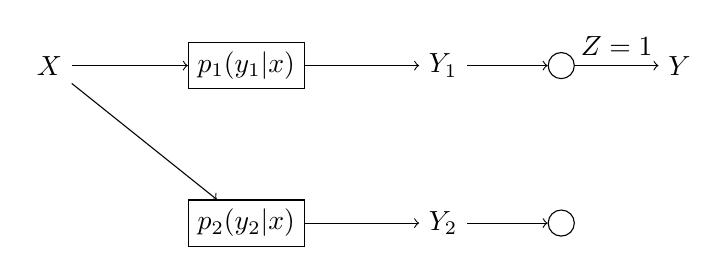
\begin{tikzpicture}[auto, node distance=2cm]

    % Nodes
    \node (X) at (0,0) {$X$};
    \node [draw, rectangle, right of=X, node distance=2.5cm] (p1) {$p_1(y_1|x)$};
    \node [draw, rectangle, below of=p1, node distance=2cm] (p2) {$p_2(y_2|x)$};
    \node [right of=p1, node distance=2.5cm] (Y1) {$Y_1$};
    \node [right of=p2, node distance=2.5cm] (Y2) {$Y_2$};
    \node [draw, circle, right of=Y1, node distance=1.5cm] (Z1) {};
    \node [draw, circle, right of=Y2, node distance=1.5cm] (Z2) {};
    \node [right of=Z1, node distance=1.5cm] (Y) {$Y$};

    % Arrows
    \draw[->] (X) -- (p1);
    \draw[->] (X) -- (p2);
    \draw[->] (p1) -- (Y1);
    \draw[->] (p2) -- (Y2);
    \draw[->] (Y1) -- (Z1);
    \draw[->] (Y2) -- (Z2);
    \draw[->] (Z1) -- node[above] {$Z=1$} (Y);

\end{tikzpicture}
\newline
a) Show that \[
I(X;Y)=\lambda I(X;Y_1) + (1-\lambda)I(X;Y_2).
\]
\begin{proof}
    \begin{align*}
        I(X;Y) &= I(X;Y,Z)-I(X;Z|Y)\\
        &=I(X;Y,Z) \quad \text{$Z$ determined by $Y$ because $\Y_1$ $\Y_2$ disjoint.}\\
        &= I(X;Z) + I(X;Y|Z)\\
        &=0+ \lambda I(X;Y_1) + (1-\lambda) I(X;Y_2)
    \end{align*}
\end{proof}
b) The capacity of the system is given by $C=\max_{p(x)}I(X;Y)$. Show that $C\leq \lambda C_1 + (1-\lambda) C_2$, where $C_i=\max_{p(x)}I(X;Y_i)$ is the capacity of the channel with transition matrix $p_i(y_i|x), i=1,2$.
\begin{proof}
    \begin{align*}
        C&= \max_{p(x)}I(X;Y)\\
        &= \max_{p(x)}(\lambda I(X;Y_1) + (1-\lambda)I(X;Y_2))\\
        &\leq \max_{p(x)}\lambda I(X;Y_1) + \max_{p(x)}(1-\lambda)I(X;Y_2)\\
        &= \lambda C_1 + (1-\lambda) C_2
    \end{align*}
\end{proof}
c) If both $C_1$ and $C_2$ can be achieved by a common input distribution, show that $C=\lambda C_1 +(1-\lambda)C_2$.
\begin{proof}
    Let $p*$ achieve both $C_1$ and $C_2$. Then by definition of $C$, $C\geq \lambda C_1 + (1-\lambda)C_2$ if we use $p*$ as the input distribution. Then, by part (b), we have equality.
\end{proof}


\subsection*{Fact about Independence}
Let $X$ and $Y$ be the input and output of a binary symmetric channel. Show that if $\epsilon=0.5$, then $X$ and $Y$ are independent.
\begin{proof}
Let $Z=1$ denote that crossover happened. 
    \begin{align*}
        P(Y=0) &= P(Y=0|X=0 Z=0)p(X=0, Z=0) + P(Y=0|X=1, Z=1)p(X=1, Z=1) \\
        &= p(X=0)p(Z=0) + p(X=1) P(Z=1)\\
        &= 0.5 
    \end{align*}
    \begin{align*}
        P(Y=0|X=0) &= P(Y=0|X=0 Z=0)p(Z=0)
        &= 0.5 
    \end{align*}
    \begin{align*}
        P(Y=0|X=1) &= P(Y=0|X=1 Z=1)p(Z=1)
        &= 0.5 
    \end{align*}
\end{proof}
\subsection*{Conditional entropy computation}
Show that $H(Y|E)=(1-\gamma)h_b(p(0))$ in the binary erasure channel.
\begin{proof}
    \begin{align*}
        H(Y|E)&=\sum_{y\in\Y}p(Y=y, E=0)\log p(Y=y|E=0)\\
        &= (1-\gamma)\sum_{y\in\Y}p(X=y)\log p(X=y)\\
        &= (1-\gamma)h_b(p(0))
    \end{align*}
\end{proof}
\end{document}